%************************************************
\chapter{The \pkgname{reshape2} package}\label{sec: reshape2}
%************************************************
\texttt{install.packages(`reshape2')}\\
\texttt{library(`reshape2')}
\bigskip 

The library \texttt{reshape} is mainly based on 
two functions: \texttt{dcast} and \texttt{melt} to
reshape the data. The former transforms a \emph{long}
data frame into a \emph{wide} one and the latter
does viceversa.
\bigskip

A long data frame is such when one (or more variables)
are arranged as row entries rather than columns instead.
If so, those variables can be re-arranged back into 
columns whose values will be function of other choses ones.
For instance, given the \texttt{quarks} data table, we can
calculate the mode (making use of the function in 
\ref{sec: functions}) for each quark in each laboratory.
The syntax is 
\texttt{dcast(dt, col1 + ... + colN \~ variable, fun.aggregate = fun)} 
\begin{verbatim}
R: dcast(quarks, lab ~flavour,  fun.aggregate = mode)
   
   Using S_z as value column.  Use the value argument 
   to cast to override this choice lab bottom charme 
   down strange  top   up

   lab bottom charme down strange  top   up
1   A   <NA>    1/2  1/2     1/2 -1/2 <NA>
2   B    1/2    1/2  1/2     1/2  1/2 <NA>
3   C    1/2    1/2  1/2     1/2  1/2  1/2
4   D    1/2    1/2  1/2    -1/2  1/2  1/2
5   E    1/2   -1/2 -1/2    -1/2  1/2 -1/2
6   F    1/2    1/2 -1/2    -1/2 <NA> -1/2
\end{verbatim}

\texttt{dcast} does not work when more than a value is
present per variable: a function must be provided
(\texttt{mode} in the example above). To illustrate
the converse behaviour we are using the in-built 
data set \texttt{airquality}.
\begin{verbatim}
R: head(airquality)

  Ozone Solar.R Wind Temp Month Day
1    41     190  7.4   67     5   1
2    36     118  8.0   72     5   2
3    12     149 12.6   74     5   3
4    18     313 11.5   62     5   4
5    NA      NA 14.3   56     5   5
6    28      NA 14.9   66     5   6
\end{verbatim}
One may want to make some of the columns row
entries instead, keeping just some others as
fixed. For instance we fix ``Month'' and 
``Day'' and melt the rest accordingly
\begin{verbatim}
melt(airquality, id.vars = c("Month", "Day")) 
 
R: head(melt(airquality, id.vars = c("Month", "Day")))
  Month Day variable value
1     5   1    Ozone    41
2     5   2    Ozone    36
3     5   3    Ozone    12
4     5   4    Ozone    18
5     5   5    Ozone    NA
6     5   6    Ozone    28

R: tail(melt(airquality, id.vars = c("Month", "Day")))
    Month Day variable value
607     9  25     Temp    63
608     9  26     Temp    70
609     9  27     Temp    77
610     9  28     Temp    75
611     9  29     Temp    76
612     9  30     Temp    68

R: data.table(melt(airquality, id.vars = 
                     c("Month", "Day")))[sample(.N,5)]
   Month Day variable value
1:     9  14     Wind  10.9
2:     7  13  Solar.R 175.0
3:     5  18     Temp  57.0
4:     5   7    Ozone  23.0
5:     8  21     Temp  77.0
\end{verbatim}
Molten data are meant to be used to plot
statistics in groups, especially histograms
for each molten variable. The below is an 
example:
\begin{verbatim}

R: iris.molten <- melt(iris, id.vars = "Species")
R: iris.molten <- data.table(iris.molten)
R: iris.molten[sample(.N,5)]

      Species     variable value
1:  virginica  Sepal.Width   2.9
2: versicolor  Sepal.Width   2.5
3:  virginica  Petal.Width   2.0
4: versicolor Sepal.Length   6.1
5:     setosa Sepal.Length   4.5

p <- ggplot(iris.molten, aes(x=value, fill = Species))
p <- p + theme(panel.grid.major = element_blank(), 
               panel.grid.minor = element_blank(),
               panel.background = element_rect(fill 
                                               = '#002b36'),
               axis.line = element_line(colour = "black"),
               legend.text=element_text(size=16),
               legend.title=element_blank(),
               axis.title.x = element_text(vjust=0, size=16),
               axis.title.y = element_text(vjust=1, size=16),
               plot.title   = element_text(vjust=1.5, size=20)) 
p <- p + geom_histogram(aes(y = ..density..), position = "dodge",
                        binwidth = 0.25, colour = "#002b36")
p <- p + facet_wrap( ~ variable, scales="free")
p <- p + guides(fill = guide_legend(override.aes = 
                                        list(colour = NULL)))
p <- p + labs(title = "Iris histograms")
p <- p + labs(x = "variable")
p <- p + labs(y = "density")
show(p)
\end{verbatim}
\begin{figure}[htbp]
 \centering
 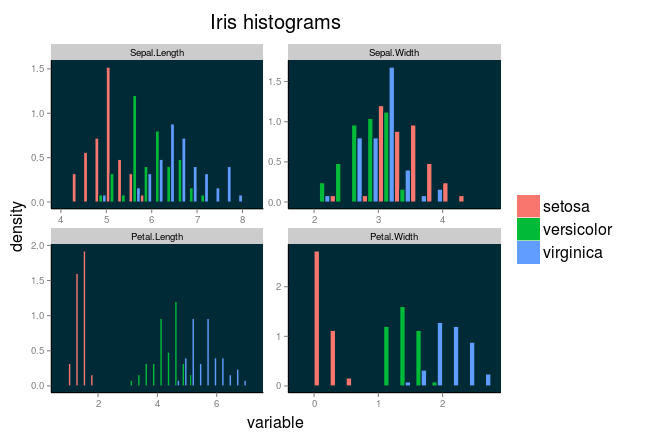
\includegraphics[scale = 0.5]{images/facet_wrap}
 \caption*{Molten data set histograms}
\end{figure}
Obviously, if we cast the molten data table 
back, we obtain the data we started with,
by definition.

\begin{verbatim}
R: dcast(melt(airquality, id.vars = c("Month", "Day")), 
        Month + Day ~ variable)
        
  Month Day Ozone Solar.R Wind Temp
1     5   1    41     190  7.4   67
2     5   2    36     118  8.0   72
3     5   3    12     149 12.6   74
4     5   4    18     313 11.5   62
5     5   5    NA      NA 14.3   56
6     5   6    28      NA 14.9   66        
\end{verbatim}




